\subsubsection{ConvLSTM}

\subsection{Autoregressive models}
Tradtional aut


\section{OLD Machine learning} \label{sec:intro_machine_learning}
In this section I will explain the computational methods used for generating the numerical experiments conducted in this thesis. Starting with the the performance metrics used to evaluate the models. Followed by the auto regressive model and recurrent neural networks. For recurrent nets I will start by explaining the simple feed forward network building up to the more complex recurrent networks. This network is also known as convolution long short-term memory network. \textbf{Anatomy and architecture.} 
\\ \\
Machine learning is a part of our daily life. From self driving bussed in  your is a word on a lot of peoples tounge. It becoming more and more a part of our daily life from search engines to googles speakers responding to speech. There are lot of different types of machine learning, suitable for solving different tasks. Figure \ref{fig:machine_learning_categories} shows the types of machine learning and their subcategories. Supervised learning is the part of machine learning concerned with learning the relation between input data, x and labelled data y. Regression predict continuous values. Replicating a function. Classification is discrete, since it assigns a category to the input. Reinforcement learning is solves games, labyrinth and fluid mechanics \textbf{(Jean Rubalt)}. Unsupervised learning tries to detect patterns in unlabelled data. This includes contains clustering and dimensionality reduction. Unsupervised and reinforcement learning is out of the scope of this thesis and will not be further discusses.
%author : Hanna Svennevik
\begin{figure}[hp]
    \centering
    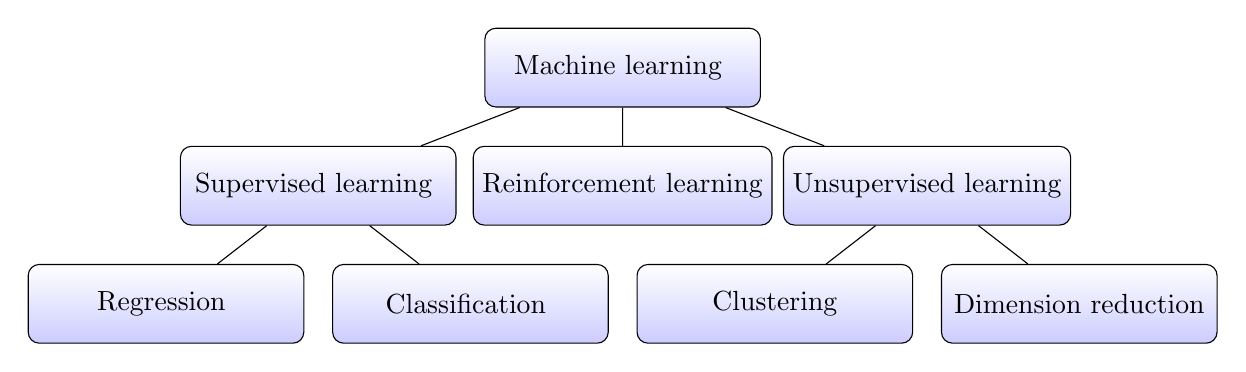
\begin{tikzpicture}[sibling distance=11em,
  every node/.style = {shape=rectangle, rounded corners,
    draw, align=center, 
    top color=white, bottom color=blue!20, minimum width=3.5cm, minimum height = 1.0cm}]]
  \node { Machine learning }
    child { node {  Supervised learning  } 
        child { node {  Regression   } }
        child { node {  Classification  } }
    }
    child {node {Reinforcement  learning}}
    child {node {Unsupervised learning}
           child { node {Clustering}}
           child { node {Dimension reduction}}};
\end{tikzpicture}
    \caption{Graph showing types of machine learning and their subcategories.}
    \label{fig:machine_learning_categories}
\end{figure}
There is a ongoing debate on what is intelligence. Traditionally a machine would be considered intelligent if it would beat a human at a given task. This has later been abandoned. The abilities a machine need to posses in order to beat a human in chess is completely different. A human needs X while the machine need Y. \textbf{kilde Chollet google} This will not be further discussed in this thesis since this is about task specific intelligence. Is it possible to train a network to gain sufficiently intelligent at the task of prediction European cloud cover?

\subsection{Supervised learning} \label{sec:supervised_learning}
Linear regression is the simplest form of supervised learning. Finding a suitable curve for a set of points. Working with real data, there is usually noise present in the dataset. In order to compensate for this we split the data into training and test (validation) sets. Overfitting becomes evident when you have a increase in the difference between the test- and training error. In non-mathematical terms, you have adjusted to much to the training data and where not able to find the general relation or "rules". See figure \ref{fig:linreg_overfitting}

\begin{figure}[hp]
    \centering
    \includegraphics{Chapter2_Theory/images/linear_regression.png}
    \caption{Fitting at different levels. The optimal fit is the most general one. This is applicable to many cases.}
    \label{fig:linreg_overfitting}
\end{figure}

\subsubsection{Autoregressive models} \label{sec:ARmodels}
The autoregressive model is a form of linear regression models where you allow a certain number of timesteps to be predictor variables. Equation \eqref{eq:AR-expression} describes how to make a prediction based on the optimal weighs, $\beta$. The expression for finding the optimal betas in a matrix form is given in equation \eqref{eq:AR-solution}. In the case for linear regression (using MSE- loss) there is only one solution to the optimal beta values. This makes it computationally very fast, as long as the matrix $X^TX$ is non-singular and thus its inverse exits. \textbf{Should i derive equation \eqref{eq:AR-solution}?}. For more complicated loss surfaces, there is no analytical solution. Gradient descent is a common algorithmn used to work around this. \textbf{write a section on gradient descent. Illustrert med mann som går ned fjellet og } 

\begin{equation} \label{eq:AR-expression}
    \hat{Y_n} = \hat{\beta_0} + \sum_{j=1}^p X_j\hat{\beta_j} + \sum_{i = 1}^{n_{ts}} Y_{n-i}\hat{\beta_{p+i}}
\end{equation}

\begin{equation} \label{eq:AR-solution}
    \hat{B} = \left( \textbf{X}^T\textbf{X} \right)^{-1}\textbf{X}\bar{y}
\end{equation}

\subsubsection{Transforming data} \label{sec:transforming_cloud_cover}
Since cloud cover fractions are in the range from zero to one, a common approach can be to transform the data so it includes values from the entire real axis $(-\infty, \infty)$. This is done using the inverse of the sigmoid function (see figure \ref{fig:sigmoid}).
% Exmale on sigmoid use this to include other plots you will use. 
\begin{figure}[hp]
    \centering
    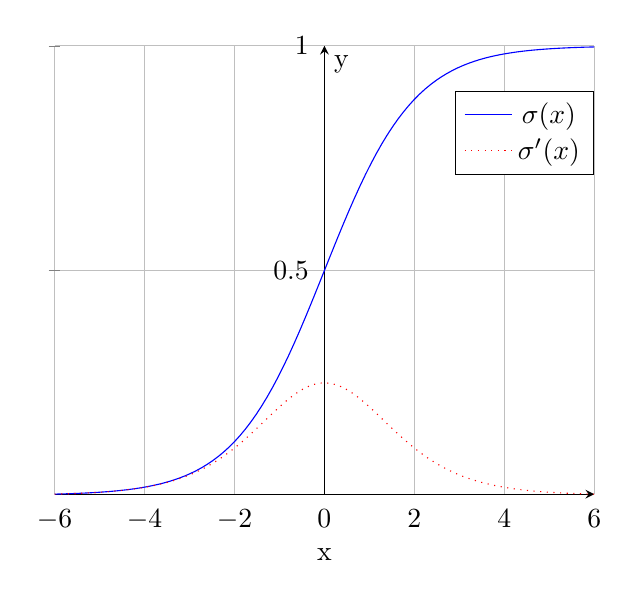
\begin{tikzpicture}[declare function={sigma(\x)=1/(1+exp(-\x));
    sigmap(\x)=sigma(\x)*(1-sigma(\x));}]
    \begin{axis}%
    [
        grid=major,     
        xmin=-6,
        xmax=6,
        axis x line=bottom,
        ytick={0,.5,1},
        ymax=1,
        ylabel= y,
        xlabel= x,
        ytick align=outside,
        ytick pos=left,
        major x tick style = transparent,
        axis y line=middle,
        samples=100,
        domain=-6:6,
        legend style={at={(1,0.9)}}     
    ]
        \addplot[blue,mark=none]   (x,{sigma(x)});
        \addplot[red,dotted,mark=none]   (x,{sigmap(x)});
        \legend{$\sigma(x)$,$\sigma'(x)$}
    \end{axis}
    \end{tikzpicture}
    
    \caption{Sigmoid function and its derivative.}
    \label{fig:sigmoid}
\end{figure}
\textbf{mer?}

\subsection{Neural network}
\begin{figure}[hp]
\centering
\def\layersep{2.5cm}
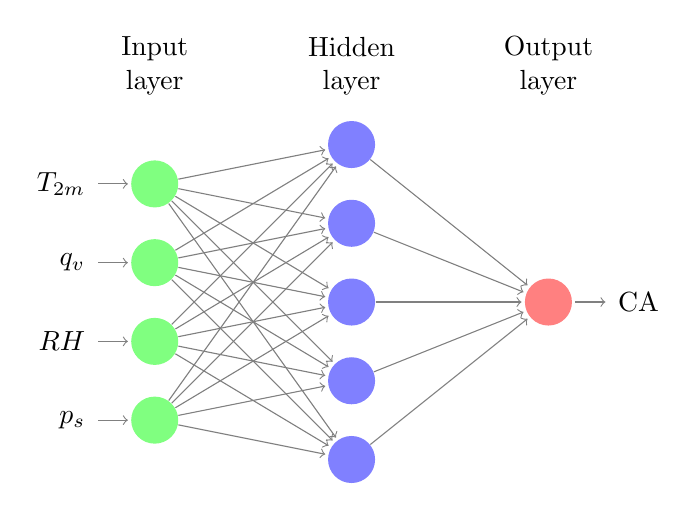
\begin{tikzpicture}[shorten >=1pt,->,draw=black!50, node distance=\layersep]
    \tikzstyle{every pin edge}=[<-,shorten <=1pt]
    \tikzstyle{neuron}=[circle,fill=black!25,minimum size=17pt,inner sep=0pt]
    \tikzstyle{input neuron}=[neuron, fill=green!50];
    \tikzstyle{output neuron}=[neuron, fill=red!50];
    \tikzstyle{hidden neuron}=[neuron, fill=blue!50];
    \tikzstyle{annot} = [text width=4em, text centered]

    \node[input neuron, pin=left:$T_{2m}$] (I-1) at (0,-1) {};
    \node[input neuron, pin=left:$q_v$] (I-2) at (0,-2) {};
    \node[input neuron, pin=left:$RH$] (I-3) at (0,-3) {};
    \node[input neuron, pin=left:$p_s$] (I-4) at (0,-4) {};

    % Draw the input layer nodes
    %\foreach \name / \y in {1,...,4}
    % This is the same as writing \foreach \name / \y in {1/1,2/2,3/3,4/4}
    %    \node[input neuron, pin=left:Input \#\y] (I-\name) at (0,-\y) {};

    % Draw the hidden layer nodes
    \foreach \name / \y in {1,...,5}
        \path[yshift=0.5cm]
            node[hidden neuron] (H-\name) at (\layersep,-\y cm) {};

    % Draw the output layer node
    \node[output neuron,pin={[pin edge={->}]right:CA}, right of=H-3] (O) {};

    % Connect every node in the input layer with every node in the
    % hidden layer.
    \foreach \source in {1,...,4}
        \foreach \dest in {1,...,5}
            \path (I-\source) edge (H-\dest);

    % Connect every node in the hidden layer with the output layer
    \foreach \source in {1,...,5}
        \path (H-\source) edge (O);

    % Annotate the layers
    \node[annot,above of=H-1, node distance=1cm] (hl) {Hidden layer};
    \node[annot,left of=hl] {Input layer};
    \node[annot,right of=hl] {Output layer};
\end{tikzpicture}

\caption{One layer hidden neural network. Taking temperature, humidities and pressure as input and estimating a fractional cloud cover - cloud amount - CA}
\label{fig:one_layer_mlp}
\end{figure}
Figure \ref{fig:one_layer_mlp} shows a simple architecture of a neural network. This consist of four input nodes or neurons, one for each of the variables relevant for the problem at hand. This is a fully connected network, meaning that every input node has a connection/weight to the next layer. After the input data has been passed to the hidden layer (sum over the matrix multiplication of the data and weight) it goes though a activation. The activation function in neural networks introduce the non-linearity's. Without then this would be piece-wise linear functions\textbf{..?}. Figure \ref{fig:activation_one_node} illustrates the activation in one node based on the input of variables. 
\begin{figure}[hp]
\centering
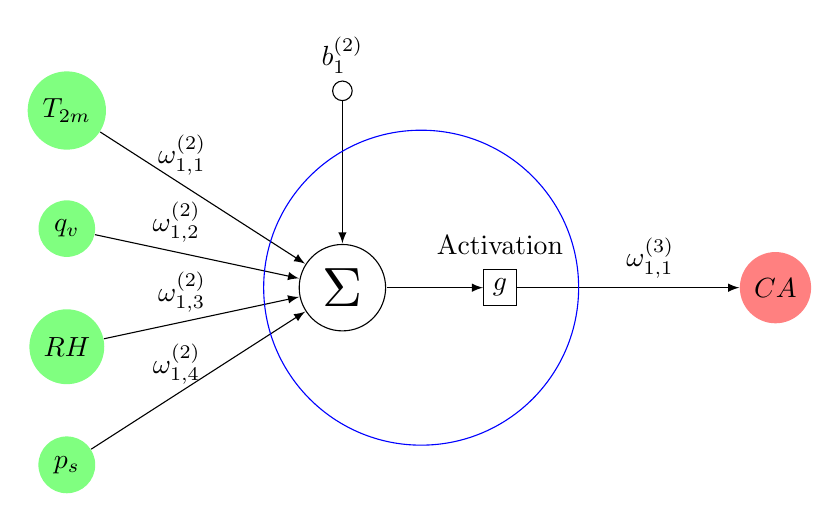
\begin{tikzpicture}[>=latex]
\path
(0,0)     node[circle,draw,scale=2,inner sep=2pt] (S) {$\Sigma$}
+(90:2.5) node[circle,draw,inner sep=2.5pt] (b) {}
          node[above=1mm] {$b_1^{(2)}$}
+(-3.5,2.25)  node[circle,fill=green!50]  (x1) {$T_{2m}$}
+(-3.5,0.75)    node[circle,fill=green!50]  (x2) {$q_v$}
+(-3.5,-0.75) node[circle,fill=green!50]  (x3) {$RH$}
+(-3.5,-2.25) node[circle,fill=green!50]  (x4) {$p_s$}
(2,0)    node[draw] (g) {$g$} node[above=3mm]{Activation}
+(3.5,0)  node[circle,fill=red!50]  (y1) {$CA$};
%+(-15:3) node[circle,fill=red!50]  (y2) {$\hat{y}_2$};
\draw[->] (S)--(g);
\draw[->] (b)--(S);
\draw[->] (g)--(y1) node[pos=.6,above]{$\omega_{1,1}^{(3)}$};
%\draw[->] (g)--(y2) node[pos=.6,below]{$\omega_{2,1}^{(3)}$};
\draw[->] (x1)--(S) node[pos=.4,above]{$\omega_{1,1}^{(2)}$};
\draw[->] (x2)--(S) node[pos=.4,above]{$\omega_{1,2}^{(2)}$};
\draw[->] (x3)--(S) node[pos=.4,above]{$\omega_{1,3}^{(2)}$};
\draw[->] (x4)--(S) node[pos=.4,above]{$\omega_{1,4}^{(2)}$};
\draw[blue] (1,0) circle(2);
\end{tikzpicture}

\caption{Sketch of the activation on one of the nodes in the hidden layer. Edit figure to have one output node. Consider using another subscript than g for activation function..?}
\label{fig:activation_one_node}
\end{figure}
In a neural network the connections between the nodes and the biases of the nodes need to be trained. This means that the optimal first layer in three layer model, is not equal to the optimal first layer in a two layer model. 
\\ \\
Three important concepts to every model. The weights, loss-function and optimiser. \textbf{neurons..?} The models is built from weights. The loss is a measure on how close you are to what you want to learn. Optimiser updates/adjust the weights in the direction of a lower loss. \textbf{Backpropagation is the learning algorithmn?} 
\begin{equation} \label{eq:relating_cc_as_a_func}
    tcc = f(T_{2m}, q_v, RH, sp)
\end{equation}
The rules I hope to achieve in this thesis is the physical relation of total cloud cover based on temperature, pressure and humidity. Like described in equation  \eqref{eq:relating_cc_as_a_func}.

Explain Difference between a neural network used for classification and regression, is choises in cost-function and activation function in the output layer (linear for regression and softmax for classification). 

\subsection{Recurrent networks}
Introduction to recurrent networks. 

\subsubsection{Convolution}
Convolution is a mathematical operation where you move a filter across you two dimensional data. Here the result in one cell is the affected by its neighbours. In a convolution neural network the trained weights are the filters. 
% kilde https://tex.stackexchange.com/questions/522118/visualizing-matrix-convolution 
\begin{figure}[hp]
    \centering
    \begin{tikzpicture}[mmat/.style={matrix of math nodes,column sep=-\pgflinewidth/2,
   row sep=-\pgflinewidth/2,cells={nodes={draw,inner sep=2pt,thin}},draw=#1,thick,inner sep=0pt},
   mmat/.default=black,
   node distance=0.3em]
 \matrix[mmat](mat1){
         0 & 1 & 1 & 1 & 0 & 0 & 0 \\ 
         0 & 0 & 1 & 1 & 1 & 0 & 0 \\ 
         0 & 0 & 0 & 1 & 1 & 1 & 0 \\ 
         0 & 0 & 0 & 1 & 1 & 0 & 0 \\ 
         0 & 0 & 1 & 1 & 0 & 0 & 0 \\ 
         0 & 1 & 1 & 0 & 0 & 0 & 0 \\ 
         0 & 1 & 0 & 0 & 0 & 0 & 0 \\ 
         };
 \node[fit=(mat1-1-4)(mat1-3-6),inner sep=0pt,draw,red,thick](f1){};        
 \node[right=of mat1] (mul) {$*$};      
 \matrix[mmat=blue,fill=blue!20,right=of mul](mat2){    
     1 & 0 & 1 \\ 
     0 & 1 & 0 \\ 
     1 & 0 & 1 \\ };
 \node[right=of mat2] (eq) {$=$};       
 \matrix[mmat,right=of eq](mat3){    
     1 & 4 & 3 & |[draw=green,thick,fill=green!20,alias=4]|4 & 1 \\ 
     1 & 2 & 4 & 3 & 3 \\ 
     1 & 2 & 3 & 4 & 1 \\ 
     1 & 3 & 3 & 1 & 1 \\ 
     3 & 3 & 1 & 1 & 0 \\ 
 };
 \foreach \Anchor in {south west,north west,south east,north east}
 {\draw[blue,densely dotted] (f1.\Anchor) -- (mat2.\Anchor); 
 \draw[green,densely dotted] (4.\Anchor) -- (mat2.\Anchor);}
 \begin{scope}[on background layer]
  \fill[red!20] (f1.north west) rectangle (f1.south east);
 \end{scope}
\end{tikzpicture}
    \caption{Diagram showing a convolutional operation.}
    \label{fig:convolution}
\end{figure}

% By J. Leon, Beerware licence is acceptable...
% https://tex.stackexchange.com/questions/432312/how-do-i-draw-an-lstm-cell-in-tikz?rq=1

% used to avoid putting the same thing several times...
% Command \empt{var1}{var2}
\newcommand{\empt}[2]{$#1^{\langle #2 \rangle}$}
\begin{figure}[hp]
    \centering
    
    \begin{tikzpicture}[
    % GLOBAL CFG
    font=\sf \scriptsize,
    >=LaTeX,
    % Styles
    cell/.style={% For the main box
        rectangle, 
        rounded corners=5mm, 
        draw,
        very thick,
        },
    operator/.style={%For operators like +  and  x
        circle,
        draw,
        inner sep=-0.5pt,
        minimum height =.2cm,
        },
    function/.style={%For functions
        ellipse,
        draw,
        inner sep=1pt
        },
    ct/.style={% For external inputs and outputs
        circle,
        draw,
        line width = .75pt,
        minimum width=1cm,
        inner sep=1pt,
        },
    gt/.style={% For internal inputs
        rectangle,
        draw,
        minimum width=4mm,
        minimum height=3mm,
        inner sep=1pt
        },
    mylabel/.style={% something new that I have learned
        font=\scriptsize\sffamily
        },
    ArrowC1/.style={% Arrows with rounded corners
        rounded corners=.25cm,
        thick,
        },
    ArrowC2/.style={% Arrows with big rounded corners
        rounded corners=.5cm,
        thick,
        },
    ]

%Start drawing the thing...    
    % Draw the cell: 
    \node [cell, minimum height =4cm, minimum width=6cm, fill = green
    , opacity=0.2] at (0,0){} ;

    % Draw inputs named ibox#
    \node [gt, fill = yellow] (ibox1) at (-2,-0.75) {$\sigma$};
    \node [gt, fill = yellow] (ibox2) at (-1.5,-0.75) {$\sigma$};
    \node [gt, minimum width=1cm, fill = yellow] (ibox3) at (-0.5,-0.75) {Tanh};
    \node [gt, fill = yellow] (ibox4) at (0.5,-0.75) {$\sigma$};

   % Draw opérators   named mux# , add# and func#
    \node [operator, fill = pink] (mux1) at (-2,1.5) {$\times$};
    \node [operator, fill = pink] (add1) at (-0.5,1.5) {+};
    \node [operator, fill = pink] (mux2) at (-0.5,0) {$\times$};
    \node [operator, fill = pink] (mux3) at (1.5,0) {$\times$};
    \node [function, fill = pink] (func1) at (1.5,0.75) {Tanh};

    % Draw External inputs? named as basis c,h,x
    \node[ct, label={[mylabel]Cell state}] (c) at (-4,1.5) {\empt{c}{t-1}};
    \node[ct, label={[mylabel]Hidden state}, fill = purple, opacity =0.3] (h) at (-4,-1.5) {\empt{h}{t-1}};
    \node[ct, label={[mylabel]left:Input}, fill = blue, opacity =0.3] (x) at (-2.5,-3) {\empt{x}{t}};

    % Draw External outputs? named as basis c2,h2,x2
    \node[ct, label={[mylabel]Cell state}] (c2) at (4,1.5) {\empt{c}{t}};
    \node[ct, label={[mylabel]Hidden state}, fill = purple, opacity =0.3] (h2) at (4,-1.5) {\empt{h}{t}};
    \node[ct, label={[mylabel]left:Output}, fill = purple, opacity =0.3] (x2) at (2.5,3) {\empt{h}{t}};
    
    % Start connecting all.
    
    % Intersections and displacements are used. 
    % Drawing arrows    
    \draw [ArrowC1] (c) -- (mux1) -- (add1) -- (c2);

    % Inputs
    \draw [ArrowC2] (h) -| (ibox4) ;
    \draw [ArrowC1] (h -| ibox1)++(-0.5,0) -| (ibox1); 
    \draw [ArrowC1] (h -| ibox2)++(-0.5,0) -| (ibox2);
    \draw [ArrowC1] (h -| ibox3)++(-0.5,0) -| (ibox3);
    \draw [ArrowC1] (x) -- (x |- h)-| (ibox3);

    % Internal - possibility , rotate = 90
    \draw [->, ArrowC2] (ibox1) -- (mux1) node[midway, left] {F};
    \draw [->, ArrowC2] (ibox2) |- (mux2) node[midway, above] {I};
    \draw [->, ArrowC2] (ibox3) -- (mux2) node[midway, right] {$\Tilde{C}$};
    \draw [->, ArrowC2] (ibox4) |- (mux3) ; %node[midway, above] {b};
    \draw [->, ArrowC2] (mux2) -- (add1) ; %node[midway, above] {c};
    \draw [->, ArrowC1] (add1 -| func1)++(-0.5,0) -| (func1) ; % node[midway, above] {d};
    \draw [->, ArrowC2] (func1) -- (mux3) node[midway, right] {O};

    %Outputs
    \draw [-, ArrowC2] (mux3) |- (h2);
    \draw (c2 -| x2) ++(0,-0.1) coordinate (i1);
    \draw [-, ArrowC2] (h2 -| x2)++(-0.5,0) -| (i1);
    \draw [-, ArrowC2] (i1)++(0,0.2) -- (x2);
    %\node [cell, minimum height =4cm, minimum width=6cm, fill = pink, opacity=.8] at (0,0){\Large A} ;
    
\end{tikzpicture}
    \caption{Architecture of a \acrshort{lstm} cell. https://tex.stackexchange.com/questions/328733/how-to-draw-recurrent-neural-network for drawing multiple cells RNN.}
    \label{fig:lstm_cell}
\end{figure}


\input{Chapter2_Theory/tikz/spherical_vs_cartesian.tikz}

\begin{figure}
    \centering
    \includegraphics{Chapter2_Theory/images/classification_overfitted.png}
    \caption{Caption}
    \label{fig:classification_overfitting}
\end{figure}

Climate models are implementations of physical equations and parametrizations. After some tuning they are thought to provide the answers given a state. You can read more about climate models in section \ref{sec:climate_models}. Since Hansen et. al. 1984 \textbf{siter} first attempted to estimate the \acrfull{ecs}, reaserchers have been working on reducing the spread. 
More complex models introduce other uncertainties and they have not yet been able to reduce it sufficiently \textbf{hvordan si "nok" - uten at et blir slemt}. With data available, more complex relations can be described. This requires deeper networks and the depth in deep learning refers to the number of layers. More complex models come with a higher risk of overfitting. \textbf{Kilde book Chollet}.

\subsection{Metrics}  \label{sec:metrics}
In order to acquire a certain skill you need a measure determining how close you are. 
Use the sum of square or abosolute values in order to not penalize point on the lower side of the line. Or not having to deal with negative distances. 
\begin{equation} \label{eq:mse}
    MSE(\hat{y},\hat{\tilde{y}}) = \frac{1}{n} \sum_{i=0}^{n-1}(y_i-\tilde{y}_i)^2
\end{equation} 

\begin{equation} \label{eq:ase}
    ASE(\hat{y},\hat{\tilde{y}}) =  \sum_{i=0}^{n-1}(y_i-\tilde{y}_i)^2
\end{equation} 

\begin{equation} \label{eq:r2}
    R^2(\hat{y}, \tilde{\hat{y}}) = 1 - \frac{\sum_{i=0}^{n - 1} (y_i - \tilde{y}_i)^2}{\sum_{i=0}^{n - 1} (y_i - \bar{y})^2}
\end{equation} 
where mean value of $\hat{y}$ is defined as $\bar{y} =  \frac{1}{n} \sum_{i=0}^{n - 1} y_i$. $R^2$ describes how much of the variation in the dataset you are able to capture with your model.



\subsection{Hyperparameters - Automatic Optimization}
Keras-tuner.
\textbf{Explain all the params you tune. Might be beneficially with a figure. See Rune's MS-thesis.}



\subsubsection{Convolutional Neural Networks}
\input{Chapter2_Theory/tikz/cnn.tikz}


\paragraph{Learning algorithmns - optimizen (implementation of sequence length)} \mbox{}\\
Describe the following
\begin{enumerate}
    \item Loss, cost, performance metric? epoch batch
\end{enumerate}

From Chollet book s. 11 \textit{the fundamental trick in deep learning is to use this score (result from performance metric) as a feedback signal to adjust the value of the weights a little, in a direction that will lower the loss score for the current example. } The adjustment is the job of the optimizer, which implements backpropagation algorithmn which is the sentral learning algoritmn.
\textbf{Explain this in words.}



\subsection{Klipp og lim}


When describing shapes, do it by keras convention. Which is channel first? \textbf{Talk about working with real data and not synthetic.} In this 
\textit{Learning means finding a suitable representation of model parameters that minimize a loss function for a given set of training data samples and their corresponding targets.}
\textbf{Does the setup here resemble videos mostly? Since its a sequence of frames containing meteorological data..}

\section{Future work}
\begin{enumerate}
    \item Describe how to make parametrization to implement in CMIP6.
    \item Programming language in climate models vs python.
\end{enumerate}



\section{Deep learning - ikke den ina rettet}
\acrfull{ai} is a part of our daily lives. From face recognition unlocking your phone to self driving busses in the Oslo city centre. Speech recognition, to can tell your phone what to write in your emails. Manpulating videos. Making it look like important people are saying something else than they originally did. \\ \\
The field dates back to the fifties. When pioneers started\textit{ discussing how one could automatise tasks normally performed by humans.} Three factors determining the advances of the field; data, hardware and algorithmns. Logistic regression and Naive Bayes classifiers are examples of algorithmns that predates computers, but are still very useful to this day. Internet continuous to provide large amounts of data from Wikipedia, Flicker (tagged images) and YouTube. Advances in computational powers, such as graphical processing units, GPU's \textit{provide a environment/platform=os to learn in/on}. These where originally develop for the gaming industry, but in 2007 they realised a interface called CUDA (2007) which allows for computing \textbf{find a up to date cost and flops (floating point operations per second)}. \textbf{siter Chollet bok}
\\ \\ 
For clarity, the deep in deep learning refer to the number of layers. Moving from shallow networks to deeper ones (more than 10) algorithmic advances in gradient propagation was needed. The main advantage of using deep neural networks is that they find their own feature representations of the given data. AI promises that if you have enough data you can find any relation. However this is not always the case, you have to add noise, non stationary system (e.g. climate) and miss-labeled data. Theorem. Data always contain noise. Using supervised learning the data might be incorrectly labelled. Human makes mistake. Earth system monitoring provides a global view of variables across meteorological systems. %\textbf{Some thing about satellite era}. These large amounts of data and the flexible nature of the neural network makes is a suitable method also in geosciences. \textbf{With enough data neural networks can serve as a universal function approximate given a suitable hyper parameter tuning and input data.} 
The last couple of years reaserchers have been attempting to use this for wide range of problems like rainfall runoff modeling (krazerts), high-resolution weather forecasting (Rodrigues), Air quality forecasting (sun and liu), precipitaiton nowcasting (Shi et al) and \textbf{kanskje: LES} \textit{deep neural network based feature representation for weather data.} \textbf{lui et al }. \textbf{noe med forskjellig hell.} Another more comprehensive machine learning project is lead by Tapio Schneider at Caltech. Along with his team of technologist they have ambitions to create a earth system model using machine learning. With his team of from MIT and former employees of Microsoft and Google they hope to create a platform which can resolve clouds and hopefully reduce the spread in \acrshort{ecs}. \textbf{cite Science}

%This includes activation functions, weight initialisation and optimisation schemes. I'll get back to that in section \ref{sec:intro_machine_learning}. Other advances like batch normalisation, depth wise separable convolutions attributed to the revolution of \acrshort{ai}. 
%\begin{figure}[h]
%    \centering
%    \includegraphics{Chapter1_Intro/images/Datenvolumen_D-SDA.jpg}
%    \caption{Data volume. By the continuous earth system monitoring, meteorology/ climate science have progressed toward becoming a big data science. Observations are most used for verifying climate models and quantifying the current state of climate. \href{https://www.dlr.de/eoc/en/desktopdefault.aspx/tabid-12632/22039_read-51751}{https://www.dlr.de/eoc/en/desktopdefault.aspx/tabid-12632/22039{\_}read-51751}.}
%    \label{fig:data_volum_sat}
%\end{figure}5